\section{Fallstudie: Optische Handgestenerkennung}
\begin{figure}
    \centering
    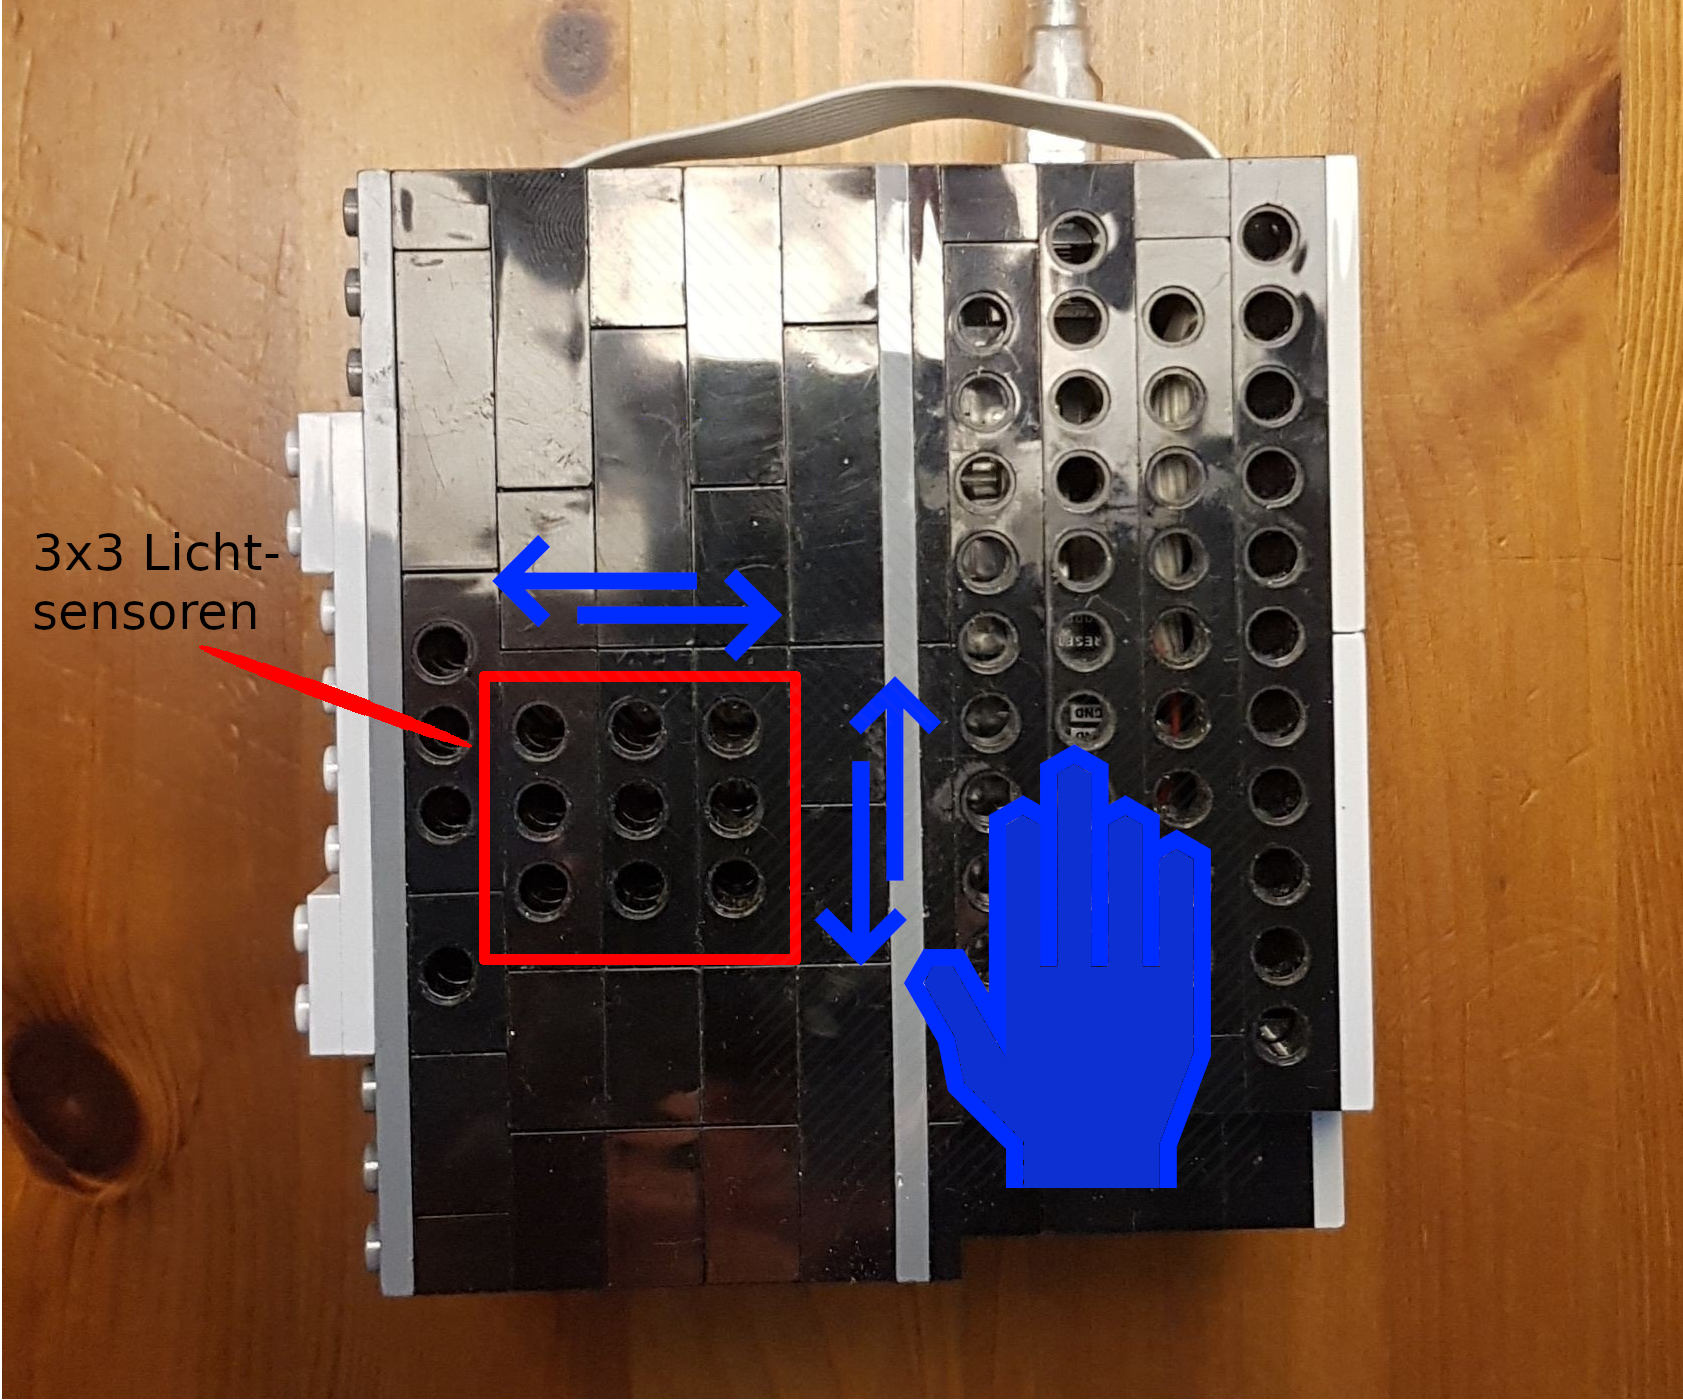
\includegraphics[width=0.6\linewidth]{images/arduino_ex.png}
    \caption{Das Arduino-Board ATmega328P mit 3x3 Matrix von Lichtsensoren in Lego-Verpackung. Illustriert werden die möglichen Handgestentypen mit Ausnahme der Nullgeste.}
    \label{fig:arduino_ex}
\end{figure}
Diese Arbeit ist Teil einer Fallstudie zur Handgestenerkennung auf Low-End Mikro-Controllern von dem Institut für Telematik an der TUHH \cite{venzkeArticle}. Das Ziel ist die Handgestenerkennung in Echtzeit mit so wenig
Resourcen wie möglich, damit die Produktion der einzelnen Module so kostengünstig wie möglich ist. Also Eingabe dient, je nach Modul, ein 3x3, bzw. 4x4, Matrix von Lichtsensoren. Dabei werden 5 Typen von Handgesten
untersucht: Links nach Rechts, Rechts nach Links, Oben nach Unten, Unten nach Oben und NullGeste, i. e. eine invalide Geste (siehe Abbildung \ref{fig:arduino_ex}).